\documentclass[UTF8,zihao=-4]{ctexart}

\usepackage[a4paper,top=2.7cm,bottom=2.5cm,left=2.7cm,right=2.7cm]{geometry}
\usepackage{graphicx}
\usepackage{amsmath}
\usepackage{booktabs}
\usepackage{tabularx}
\usepackage{array}
\usepackage{longtable}
\usepackage{caption}
\usepackage{enumitem}
\usepackage{fancyhdr}
\usepackage{xurl}
\usepackage[hidelinks]{hyperref}
\usepackage{tikz}
\usetikzlibrary{arrows.meta}

\graphicspath{{figures/}{../../figures/}}
\setlength{\parindent}{2em}
\setlength{\parskip}{0.35em}
\setlength{\headheight}{15pt}
\Urlmuskip=0mu plus 1mu
\setlist{nosep}
\captionsetup{font=small,labelfont=bf}

\pagestyle{fancy}
\fancyhf{}
\lhead{河北省城乡融合发展与乡村振兴结项报告}
\rhead{\thepage}
\renewcommand{\headrulewidth}{0.4pt}

\newcommand{\source}[1]{\par\noindent{\small\textbf{资料来源：}#1}}

\begin{document}

\begin{titlepage}
    \centering
    \vspace*{2.2cm}
    {\zihao{2}\bfseries 雄安新区城乡融合发展与乡村振兴\par}
    \vspace{0.25cm}
    {\zihao{2}\bfseries 协同路径研究\par}
    \vspace{0.8cm}
    {\zihao{3}\bfseries 结项报告\par}
    \vspace{1.5cm}
    {\zihao{4} 课题名称：河北省城乡基础设施一体化与公共服务均等化路径研究\par}
    \vspace{0.4cm}
    {\zihao{4} 所属方向：城乡融合发展与乡村全面振兴协同\par}
    \vspace{0.4cm}
    {\zihao{4} 课题负责人：王维佳\par}
    \vspace{0.4cm}
    {\zihao{4} 所在单位：石家庄金融职业学院大数据会计学院\par}
    \vfill
    {\zihao{4} 2026年6月\par}
\end{titlepage}

\tableofcontents
\newpage

\section*{摘\quad 要}
\addcontentsline{toc}{section}{摘要}

在京津冀协同发展、雄安新区建设和乡村全面振兴战略叠加背景下，河北省城乡关系正在由单向城镇化带动转向空间重构、产业协同、公共服务均等化和生态价值转化并进的新阶段。本报告以雄安新区为核心案例，兼顾全省层面统计判断和典型地区机制分析，采用描述性统计、耦合协调测度、障碍因子分析、案例分析和机制归纳方法，研究河北省城乡融合发展与乡村振兴的现实基础、运行机制和优化路径。研究发现：截至2026年4月可获得的最新统计资料显示，2025年河北省地区生产总值达49305.2亿元，常住人口城镇化率为64.54\%，城乡居民收入比缩小至2.04，农村居民收入增速快于城镇居民，城乡差距继续收敛；2011-2023年耦合协调测度表明，河北总体由濒临失调进入中级协调阶段，但尚未达到高级协调，主要短板集中于乡村产业链延伸、农村公共服务供给、空间建设质量和生态收益转化。雄安新区通过规划引领、承接疏解、公共服务重构、白洋淀生态治理、回迁群众就业创业和淀边乡村旅游，形成了“空间重构-产业导入-服务均等-农民分享”的综合机制。报告提出，河北应以县域为基本单元推进城乡基础设施一体化，以雄安新区经验带动全省分类建设城乡产业协同平台，完善数字普惠金融和政府引导型资金工具，并建立以农民收益、公共服务可及性和生态价值实现为核心的绩效评价体系。

\textbf{关键词：}雄安新区；城乡融合发展；乡村振兴；公共服务均等化；河北省

\section{研究背景、任务与方法}

\subsection{研究背景}

城乡融合发展是中国式现代化的重要空间命题。对河北省而言，这一命题具有双重战略含义：一方面，河北环绕京津，是京津冀协同发展的重要承载地，承接北京非首都功能疏解和产业外溢是推动县域发展、乡村增收的重要机遇；另一方面，河北仍是农业大省，县域数量多、乡村人口规模大，农村产业链条短、公共服务薄弱、生态功能区增收渠道不足等问题仍然制约城乡融合质量。

本报告所称“城乡融合发展”，主要指人口、土地、资本、产业、公共服务和生态资源在城乡之间的双向流动和制度衔接；所称“乡村振兴”，主要指乡村产业、生态、文化、治理和农民生活水平的整体提升。二者的关系是：城乡融合为乡村振兴提供要素流动、公共服务和市场连接条件，乡村振兴则为城乡融合提供产业承接、生态空间和共同富裕基础。

雄安新区是观察河北城乡融合发展与乡村振兴协同机制的关键窗口。与传统城市扩张不同，雄安新区以承接北京非首都功能疏解为牵引，在规划建设新城的同时推进白洋淀生态治理、回迁群众市民化、基础设施和公共服务重构、现代农业与乡村旅游发展，其过程集中呈现了河北城乡融合发展所面对的空间、产业、公共服务和农民收益问题。因此，本报告采用“全省统计判断+雄安典型案例”的结构：全省层面回答河北城乡融合处于什么阶段、短板在哪里；雄安案例回答空间重构、产业导入、公共服务均等化和乡村振兴如何在具体地区发生。本报告为课题结项汇报稿，耦合协调测度、指标体系和障碍因子结果摘编入附录，完整测度数据库和前期调研报告作为结项支撑材料一并提交。

\subsection{研究任务}

本课题围绕“河北省城乡基础设施一体化与公共服务均等化路径研究”展开，结项阶段重点完成以下任务：

\begin{enumerate}
    \item 梳理河北省城乡融合发展和乡村振兴的总体进展，形成基于最新统计资料的事实判断。
    \item 以雄安新区为核心案例，分析新区建设、承接疏解、公共服务、生态治理和乡村产业之间的协同关系。
    \item 借鉴“社会-空间”耦合和微旅游促进城乡互动等研究视角，提炼可供河北省其他地区参考的机制经验。
    \item 提出面向河北省县域城乡融合、乡村振兴和公共服务均等化的政策建议。
\end{enumerate}

\subsection{资料来源与研究方法}

本报告主要使用四类资料：第一，河北省2025年国民经济和社会发展统计公报、河北省统计局和国家统计局河北调查总队公开数据，数据截止时点为2026年4月公开发布的统计资料；第二，中国雄安官网、河北日报、雄安媒体中心等公开发布的雄安新区建设、生态治理和乡村案例资料；第三，课题组前期形成的《河北省城乡协同发展调研报告》及2011-2023年设区市面板测度数据库，原始数据来自历年《河北省统计年鉴》《中国城乡建设统计年鉴》《中国农村统计年鉴》《河北省城乡建设统计年鉴》、各设区市统计年鉴和政府工作报告；第四，用户提供的两篇参考论文，即杨贵庆等关于浙江黄岩乡村“社会-空间”更新实践的研究，以及张俏敏等关于杭州上塘古运河和日本川场村微旅游模式的比较研究。

方法上，本报告采用描述性统计、耦合协调度模型、障碍度模型、典型案例分析和机制归纳相结合的研究策略。描述性统计用于判断河北城乡融合发展的阶段特征；耦合协调度模型用于测度新型城镇化与乡村振兴两个子系统的协调水平；障碍度模型用于识别制约协同发展的关键指标；案例分析用于呈现雄安新区城乡融合发展的实践过程；机制归纳用于从雄安经验中提炼可复制、可调整的政策逻辑。模型设定、指标体系和主要测度结果见附录A、附录B。

\section{理论借鉴与分析框架}

\subsection{“社会-空间”耦合视角}

杨贵庆等以浙江黄岩为例提出，城乡链接和城乡融合的关键在于把握社会系统与空间系统的关联逻辑。其核心启示是：空间发展如果超前于社会演进，能够引导社会结构变化；社会系统变化过快而空间供给不足，则可能引发空间失序和资源配置失衡；空间发展与社会结构变化相适应时，城乡系统才能实现协同发展和互促互馈。

这一视角对雄安新区具有直接解释力。雄安新区不是单纯建设新城，而是在大规模空间建设中同步推进人口安置、就业创业、公共服务、社区治理、生态修复和产业导入。换言之，雄安的城乡融合成效，不取决于建设面积本身，而取决于新城空间是否能够承接回迁群众生活方式转变、北京疏解资源导入、白洋淀生态保护和周边乡村产业升级。

\subsection{城乡互动与微旅游视角}

张俏敏等关于微旅游模式的研究表明，微旅游对城乡协同发展的促进作用并不只在旅游收入，而在于通过短时、高频、轻体验的城乡流动，打破城乡之间的空间壁垒、认知壁垒和消费壁垒。其案例启示包括：以城市更新提升供给质量，以乡村振兴提高乡村供给效能，以城乡互动构建复合型供给体系，并通过数字化、夜间经济、研学体验、农业认养等方式增强城乡连接。

这一视角有助于理解雄安新区白洋淀淀边乡村的转型路径。七间房乡等案例说明，生态治理形成的水清岸绿和鸟类回归，为乡村旅游、农特产品、文化体验和民宿发展提供了基础；但能否转化为强村富民，取决于是否建立统一运营、规范管理、收益分享和生态保护约束并重的制度安排。

\subsection{本报告分析框架}

综合上述理论，本报告将雄安新区城乡融合发展概括为五个环节：一是以新区规划和基础设施建设重构城乡空间；二是以承接北京非首都功能疏解导入产业、资本和人才；三是以教育、医疗、养老和社区治理提升公共服务均等化水平；四是以白洋淀生态治理和乡村旅游推进生态价值实现；五是以就业、创业、产业、物业“四业并举”和承包地、宅基地、集体经营性用地“三块地”改革拓宽群众收入来源。其中，空间重构和公共服务重构用于检验“空间建设必须匹配社会适应条件”的命题，生态旅游和智慧农业案例用于检验“城乡高频互动必须形成收益分享机制”的命题，政策建议则围绕空间、产业、服务、生态和收益五个环节展开。其逻辑框架见图\ref{fig:framework}。

\begin{figure}[htbp]
    \centering
    \begin{tikzpicture}[
        >=Stealth,
        font=\small,
        box/.style={draw, rounded corners=3pt, align=center, thick, minimum height=1.05cm},
        gov/.style={box, draw=blue!70, fill=blue!5, minimum width=2.75cm},
        market/.style={box, draw=green!60!black, fill=green!5, minimum width=2.75cm},
        platform/.style={box, draw=orange!85!black, fill=orange!6, minimum width=3.45cm, minimum height=1.45cm},
        casebox/.style={box, draw=gray!70, fill=gray!8, minimum width=2.75cm},
        result/.style={box, draw=purple!70, fill=purple!6, minimum width=2.45cm, minimum height=1.65cm}
    ]
        \node[gov] (gov) at (0,2.2) {政府赋能\\规划、资金、制度};
        \node[market] (market) at (0,-1.8) {市场运营\\企业、资本、平台};
        \node[platform] (platform) at (4.0,0.2) {城乡产业协同平台\\特色镇、小城镇、农业园区\\美丽乡村、融合项目};
        \node[casebox] (xiongan) at (8.1,2.2) {雄安新区\\空间引领型};
        \node[casebox] (baiyangdian) at (8.1,0.2) {白洋淀片区\\生态旅游型};
        \node[casebox] (county) at (8.1,-1.8) {县域农业园区\\产业链延伸型};
        \node[result] (result) at (11.8,0.2) {城乡协同结果\\就业增加\\收入提升\\公共服务改善};
        \draw[->, thick, blue!70] (gov.east) -- (platform.north west);
        \draw[->, thick, green!60!black] (market.east) -- (platform.south west);
        \draw[->, thick, orange!85!black] (platform.east) -- (xiongan.west);
        \draw[->, thick, orange!85!black] (platform.east) -- (baiyangdian.west);
        \draw[->, thick, orange!85!black] (platform.east) -- (county.west);
        \draw[->, thick, purple!70] (xiongan.east) -- (result.north west);
        \draw[->, thick, purple!70] (baiyangdian.east) -- (result.west);
        \draw[->, thick, purple!70] (county.east) -- (result.south west);
        \node[align=center, text=gray!75, font=\footnotesize] at (5.9,-3.05)
        {案例逻辑：不同区域选择不同平台形态，但共同依赖“政府降低风险 + 市场提升效率 + 农民分享收益”。};
    \end{tikzpicture}
    \caption{城乡融合发展的机制框架}
    \label{fig:framework}
\end{figure}

\section{河北省城乡融合发展与乡村振兴的现实基础}

\subsection{城乡收入差距继续收敛}

从最新统计看，河北省城乡关系已出现持续改善。2025年，河北省地区生产总值为49305.2亿元，按不变价格计算比上年增长5.6\%；常住人口城镇化率为64.54\%，比上年末提高1.12个百分点；居民人均可支配收入36439元，增长5.1\%。按常住地分，城镇居民人均可支配收入47544元，增长4.2\%；农村居民人均可支配收入23319元，增长5.9\%。城乡居民人均可支配收入比值为2.04，比上年缩小0.03。

\begin{table}[htbp]
    \centering
    \caption{河北省城乡融合发展主要统计指标}
    \label{tab:hebei-indicators}
    \begin{tabularx}{\textwidth}{>{\raggedright\arraybackslash}p{3.6cm}ccc>{\raggedright\arraybackslash}X}
        \toprule
        指标 & 2011年 & 2023年 & 2025年 & 数据说明 \\
        \midrule
        常住人口城镇化率 & 45.6\% & 64.4\% & 64.54\% & 2011年、2023年来自课题组根据《河北省统计年鉴》整理；2025年来自《河北省2025年国民经济和社会发展统计公报》。 \\
        农村居民人均可支配收入 & 7119元 & 18938元 & 23319元 & 2011年、2023年来自课题组根据《河北省统计年鉴》整理；2025年来自《河北省2025年国民经济和社会发展统计公报》。 \\
        城乡居民收入比 & 2.43 & 2.26 & 2.04 & 2011年、2023年由城镇、农村居民人均可支配收入计算；2025年统计公报直接披露为2.04。 \\
        \bottomrule
    \end{tabularx}
    \source{课题组根据《河北省统计年鉴》、前期测度数据库和《河北省2025年国民经济和社会发展统计公报》整理。}
\end{table}

表\ref{tab:hebei-indicators}显示，河北城乡收入差距收敛具有两个特点。第一，农村居民收入增长快于城镇居民，说明乡村端追赶效应仍在延续。第二，城乡收入比由2011年的2.43降至2025年的2.04，表明城乡收入差距出现较明显收敛。另据2025年统计公报，全省地区生产总值为49305.2亿元，县域地区生产总值为27199.6亿元，县域经济仍是城乡融合发展的重要承载空间。但是，收入比下降并不自动意味着城乡融合质量同步提高，仍需观察产业、公共服务、生态收益和空间建设质量等维度。

\begin{figure}[htbp]
    \centering
    
\includegraphics[width=0.86\textwidth]{report_urban_income_clean.png}
    \caption{河北省城镇化率提升与城乡收入比收敛}
    \label{fig:urban-income}
    \caption*{\footnotesize\textbf{资料来源：}课题组根据《河北省统计年鉴》及前期测度数据库绘制。}
\end{figure}

\subsection{城乡协同综合发展水平处于中级协调阶段，主要短板可由障碍度识别}

前期测度结果显示，2011-2023年河北城乡耦合协调度由0.484提高至0.677，整体由濒临失调进入中级协调阶段，但尚未跨越0.7的高级协调门槛。从空间格局看，唐山、石家庄、廊坊等区位和产业基础较好的地区协调水平较高，张家口、承德等生态功能较强地区协调水平相对偏低。这说明河北城乡融合的难点不在于是否推进城镇化，而在于如何提升乡村端的产业承接能力、公共服务承载能力和生态价值转化能力。

\begin{figure}[htbp]
    \centering
    
\includegraphics[width=0.86\textwidth]{report_coupling_clean.png}
    \caption{河北省城乡耦合协调度演进}
    \label{fig:coupling}
    \caption*{\footnotesize\textbf{资料来源：}课题组根据2011-2023年设区市面板测度结果绘制，模型说明见附录A。}
\end{figure}

\subsection{短板集中于产业链、公共服务和空间质量}

障碍因子分析显示，2023年河北城乡协同发展的主要短板集中于农产品加工转化不足、农村卫生服务供给不足、公共财政能力差异、土地生产率偏低和建成区扩张质量约束。2025年统计公报也从侧面印证了这一判断：全省乡村消费品零售额2460.1亿元，增长3.6\%，低于城镇消费品零售额6.0\%的增速；全年接待国内游客和旅游总花费虽分别增长10.9\%和10.2\%，但乡村旅游、生态旅游和县域消费能否稳定转化为农民收入，仍取决于经营主体、交通节点、品牌运营和收益分配机制。

\begin{figure}[htbp]
    \centering
    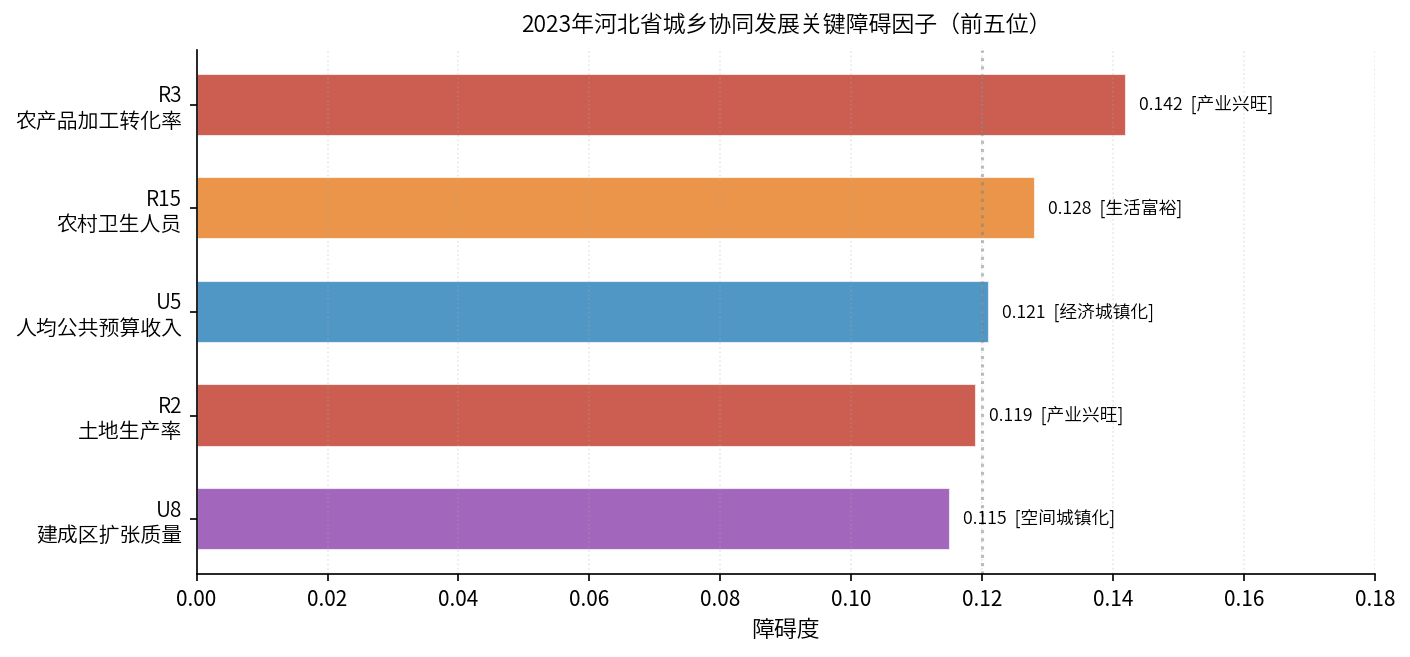
\includegraphics[width=0.86\textwidth]{report_obstacles_clean.png}
    \caption{河北城乡协同发展的关键障碍因子}
    \label{fig:obstacles}
    \caption*{\footnotesize\textbf{资料来源：}课题组根据2023年障碍度模型测算结果绘制，完整数值见附录B。}
\end{figure}

\section{雄安新区城乡融合发展与乡村振兴的实践分析}

\subsection{空间重构：从县域乡村到未来城市}

雄安新区地处北京、天津、保定腹地，距离北京、天津均约105公里，距北京大兴国际机场约55公里，规划面积1770平方公里，其中起步区规划面积198平方公里、启动区规划面积38平方公里。新区的空间意义不只是新增一座城市，而是通过高标准规划和基础设施建设，为京津冀区域要素重组和河北城乡融合发展提供战略载体。

“十四五”以来，雄安新区每年保持约2000亿元投资规模，累计完成投资工作量超过10000亿元，地区生产总值年均增长17.1\%。截至2025年11月，新区总开发面积覆盖近215平方公里，5300多栋楼宇建成或拔地而起，入廊管线超过1000公里，城市开发由点状、线性工程转向集中连片、组团式建设。这一过程为回迁安置、产业承接、公共服务配置和乡村片区更新提供了空间基础。按照“社会-空间”耦合视角，雄安案例说明，空间先行并非单纯扩张建设用地，而是通过确定性的规划和基础设施供给，引导人口安置、产业迁入和公共服务重组同步发生。

\begin{table}[htbp]
    \centering
    \caption{雄安新区城乡融合发展相关事实}
    \label{tab:xiongan-facts}
    \begin{tabularx}{\textwidth}{>{\raggedright\arraybackslash}p{3.5cm}>{\raggedright\arraybackslash}X}
        \toprule
        维度 & 主要事实与来源说明 \\
        \midrule
        规划范围 & 规划面积1770平方公里，起步区198平方公里，启动区38平方公里；数据来自中国雄安官网“大美雄安”概况页。 \\
        建设进展 & “十四五”以来累计完成投资工作量超过10000亿元，每年保持约2000亿元投资规模；总开发面积覆盖近215平方公里，5300多栋楼宇建成或拔地而起，入廊管线超过1000公里；数据来自中国雄安官网2025年11月15日报道。 \\
        承接疏解与民生服务 & 400多家央企分支机构、4000多家北京来源企业落地雄安；平稳有序安置16.9万名回迁群众，新建中小学和幼儿园105所；数据来自中国雄安官网“大美雄安”概况页。 \\
        生态治理 & 白洋淀水质稳定保持在III类，野生鸟类296种，较新区设立前增加90种，森林覆盖率由11\%提升至35.1\%；数据来自中国雄安官网“大美雄安”概况页和白洋淀水质相关报道。 \\
        \bottomrule
    \end{tabularx}
    \source{中国雄安官网“大美雄安”概况页、2025年11月15日《雄安新区累计完成投资工作量超10000亿元》等公开报道。}
\end{table}

\subsection{产业导入：承接疏解带动就业和创新要素集聚}

雄安新区的产业发展逻辑不同于一般产业园区招商。新区首先承担北京非首都功能疏解集中承载地功能，通过总部机构、高校、医院、科研平台和央企分支机构集聚，带动人才、资本、技术和高端服务要素进入河北。公开资料显示，首批疏解的中国星网、中国华能、中国中化总部入驻运营，中国矿产总部主体结构封顶，首批4所高校、2家医院全面建设；第二批疏解项目有序开工；400多家央企分支机构、4000多家北京来源企业落地雄安。

对乡村振兴而言，产业导入的关键不是企业数量本身，而是就业和收入渠道能否向回迁群众和周边农村居民延伸。新区提出就业、创业、产业、物业“四业并举”，并通过工资性、投资性、财产性、转移性“四项收入”拓宽群众增收渠道。这与传统征迁安置不同，其核心在于使农民从土地依赖型收入结构，逐步转向就业收入、经营收入、财产收益和公共服务福利共同支撑的市民化收入结构。

从理论框架看，产业导入对应“空间发展引导社会结构变化”的过程：只有当产业岗位、技能培训和社区就业服务同步进入新城空间时，承接疏解资源才会从建筑和机构层面的“落地”转化为居民就业和收入结构的改善。

\subsection{公共服务重构：从安置住房到“15分钟生活圈”}

公共服务均等化是城乡融合能否真正落地的关键。雄安新区平稳有序安置16.9万名回迁群众，新建中小学和幼儿园105所，北京四中、人大附中、疏解高校附中牵头集团化办学，雄安宣武医院运营良好。社区层面，容东、容西、雄东等片区逐步形成教育、医疗、养老、文化活动和便民服务综合配置的“15分钟生活圈”。

从“社会-空间”耦合视角看，回迁群众从村庄进入新型社区，并不是简单的居住地点变化，而是生活方式、社会交往、就业结构和治理关系的同步转变。公共服务供给如果跟不上，空间建设容易导致社会适应压力；如果公共服务、就业创业和社区治理同步推进，回迁安置就能成为城乡融合和共同富裕的制度入口。

\subsection{生态治理：白洋淀修复与生态价值转化}

白洋淀是雄安新区生态底色，也是河北城乡融合发展中生态价值转化的典型场景。公开资料显示，白洋淀水质自2021年首次达到III类标准以来持续稳定保持良好状态，野生鸟类达到296种，较新区设立前增加90种；鱼类恢复至50种。新区通过清淤疏浚、百淀连通、退耕还淀、科学补水和严密防洪等工程，推动“华北明珠”生态系统修复。

生态治理对乡村振兴的意义有两层。第一，改善农村人居环境和生态安全，提升居民福利。第二，为乡村旅游、生态研学、农特产品、文化体验等新业态提供价值基础。需要注意的是，生态价值转化不能以过度商业化破坏生态修复成果，必须在限流、准入、统一运营和收益分享机制下推进。

这体现了微旅游视角中的边界条件：生态空间能够吸引城市居民短时高频进入乡村，但只有在环境容量、运营主体和收益分配规则清晰的情况下，城乡互动才不会演变为对生态资源的消耗。

\subsection{乡村产业案例一：七间房乡生态旅游强村富民}

七间房乡位于雄县南部，11个行政村沿千里堤分布，拥有1.8万亩白洋淀水域。近年来，该乡依托白洋淀生态修复和乡村游秩序整治，探索“统一运营管理、分散服务创收”模式，建设游客服务中心、标准化泊位和智能售票系统，精选5个基础较好的村成立旅游公司，将171艘船舶纳入规范化管理。

这一模式已经形成较明确的收益结果。2024年数据显示，5个村集体公司每年接待游客11.6万人次，创造旅游综合收入374.48万元，带动5个村村集体经济累计增收55.8万元，平均每村增收约11.2万元。该案例的启示是，乡村旅游不是“各家各户自发揽客”，而应通过统一运营、规范船只、统一线路价格、村集体公司参与和生态限流，把旅游流量转化为村集体收益和农户就业收益。

从微旅游促进城乡互动的视角看，七间房乡案例验证并补充了”城乡高频互动必须形成收益分享机制”这一命题的内在逻辑：城市游客的短时高频进入本身并不能自动产生强村富民效果，只有当收益分配规则（统一运营、村集体参与、船只规范纳管）和环境限制（生态限流、游线管控）先于大规模引流建立起来，城乡流动才能从消费活动转化为可持续的村集体经济收入。若缺乏规则先行，微旅游流量容易形成”利润外流、风险内留”的逆向分配，与共同富裕目标相悖。

\subsection{乡村产业案例二：安新县智慧农业场景}

安新县阳雀湖西里现代农业产业园区展现了雄安新区乡村振兴的另一类路径。该园区在1100亩土地上建设66座暖棚、96座冷棚和8座圆形拱棚，通过远程可控、无土栽培、数据化管理等方式推进农业生产智能化，并实现“南椒北种”等品种和技术场景融合。

与淀边旅游相比，智慧农业的重点在于把乡村资源从初级种植环节推向设施农业、数字管理、品牌经营和稳定订单。对河北其他地区而言，安新经验表明，农业现代化不是简单扩大种植面积，而是通过设施、技术、数据、金融和市场渠道提升单位土地产出和经营稳定性。

从”社会-空间”耦合视角看，安新案例说明，当设施农业的技术导入（空间更新：暖棚建设、无土栽培、数字管控）与农户技能培训、订单农业组织、品牌运营等社会系统变化同步推进时，乡村生产空间才能真正承接更高附加值的市场需求，实现”空间升级驱动社会收益”的正向耦合；若技术设施先行而社会端——农户经营能力、稳定市场渠道、金融支持——未能同步跟进，空间投入将难以转化为稳定农业收益，导致”有设施、无效益”的空间-社会错位。这也提示，衡量智慧农业项目成效的核心指标，不应止步于土地利用率或产量，还须纳入农户组织化程度、订单稳定性和净收益分配结构。

\section{雄安案例揭示的运行机制}

\subsection{规划引领机制：用空间确定性降低市场和社会不确定性}

雄安新区坚持“一张蓝图绘到底”，通过国土空间规划、交通网络、生态廊道、地下管廊和数字城市同步建设，为产业导入和公共服务配置提供了稳定预期。规划引领的作用不只是控制建设秩序，更在于减少市场主体和居民对未来空间功能的不确定性，使产业、住房、学校、医院、生态空间和乡村片区能够形成相互支撑。

\subsection{平台承接机制：把外部资源转化为本地发展能力}

北京非首都功能疏解带来的总部、科研、教育、医疗和企业资源，只有通过新区平台、产业载体、社区服务和县域乡村项目承接，才能转化为河北本地发展能力。雄安的经验说明，平台不是单个项目，而是政府、企业、村集体、社区组织和公共服务机构之间的组织网络。没有平台，外部资源容易停留在城市建设层面；有了平台，外部资源才能进入就业、产业链、公共服务和村集体经济。

\subsection{公共服务均等化机制：以服务重构促进市民化}

城乡融合不能只看收入和建设规模，还要看教育、医疗、养老、文化和社区治理是否能够支持农民稳定融入城市生活。雄安新区新建学校、引入优质教育集团、建设医疗机构和社区服务体系，实际上是在为“村民向市民转变”提供制度条件。这一机制对河北其他地区具有普遍意义：县域城镇化和乡村振兴必须同步推进公共服务均等化，否则人口流动和空间重构难以稳定。

\subsection{生态价值实现机制：从生态治理到强村富民}

白洋淀治理使水质、鸟类、鱼类和湿地景观持续改善，为生态旅游和生态产品价值实现创造基础。七间房乡案例进一步表明，生态价值只有通过规范经营和收益分享才能成为强村富民的现实收入。生态功能区不能简单复制工业园区模式，应当以生态保护红线、游客容量控制、村集体运营、农户就业和文旅品牌建设为核心，形成“保护越好、收益越稳”的正向激励。

\subsection{农民分享机制：以就业和财产收益评价协同成效}

雄安新区回迁安置和“四业并举”表明，城乡融合政策的核心评价对象应当是群众能否获得稳定收益。农民分享收益至少包括四类：工资性收入，即通过新区建设、服务业、社区岗位和产业平台就业；经营性收入，即参与民宿、餐饮、农特产品和乡村旅游；财产性收入，即土地、房屋、村集体资产和经营性用地收益；公共服务收益，即教育、医疗、养老和社区服务改善带来的福利提升。

\section{存在问题与风险判断}

\subsection{乡村产业收益规模仍需扩大}

七间房乡生态旅游已经形成较好示范，但从11.6万人次游客、374.48万元旅游综合收入和55.8万元村集体增收看，其规模仍处于起步阶段。若要成为稳定增收渠道，还需要延长消费链条，增加餐饮、住宿、研学、文创、农产品销售和夜间消费等复合业态，同时防止同质化和过度商业化。

\subsection{回迁群众社会适应和就业质量仍需长期跟踪}

16.9万名回迁群众进入新型社区，意味着生产生活方式发生深刻变化。短期内可以通过公共岗位、社区服务和建设就业实现托底，但长期看仍需提高技能培训、产业吸纳和创业支持质量，避免就业低端化、收入不稳定和社区治理压力累积。

\subsection{公共服务均等化需要从“有设施”转向“高质量运营”}

学校、医院、养老设施和社区服务设施建成后，关键在于师资、医生、护理、运营管理和财政可持续。尤其是新区新建片区与保留村庄、淀区村庄之间，公共服务供给质量可能存在差异。未来应从设施均等化进一步转向服务质量均等化和可及性均等化。

\subsection{生态保护与旅游开发之间需要动态平衡}

白洋淀水质稳定保持III类、野生鸟类增加，是雄安新区最重要的生态资本。随着旅游热度上升，若游客容量、船舶排放、岸线开发和餐饮民宿管理不到位，可能对生态系统造成压力。因此，生态旅游必须坚持限流、绿色交通、统一码头、污水垃圾治理和生态监测同步推进。

\section{政策建议}

前文的统计测度和案例分析表明，河北城乡融合发展的主要约束并不在单一指标，而在于“乡村端承接能力不足”：产业链延伸不足、农村公共服务短板、生态价值转化机制不稳、回迁和人口流动后的社会适应压力并存。因此，政策设计应从一般性项目建设转向“基础设施一体化、公共服务均等化、产业平台化、金融工具适配化和绩效评价结果化”的组合方案，并根据环京津、冀中南、冀东、冀北不同区域条件分类推进。

\subsection{以县域为基本单元推进城乡基础设施一体化}

河北应把县域作为城乡融合发展的基本实施单元，统筹县城、小城镇、中心村和特色村的道路、供水、污水、垃圾、数字网络、冷链物流和公共服务设施。对接雄安经验，各地不宜简单追求大规模新城建设，而应根据人口集聚趋势和产业基础，形成“县城综合服务中心-重点镇产业节点-中心村生活服务节点-特色村生态文旅节点”的分级体系。环雄安和环京津地区应优先补齐通勤交通、公共服务同城化和产业配套设施；冀中南地区应优先建设农产品冷链、加工园区和县域物流节点；冀北生态功能区应优先完善生态旅游交通、清洁能源接网、污水垃圾治理和数字通信设施，避免套用高强度工业园区模式。

\subsection{以公共服务均等化提升乡村人口留存能力}

城乡融合的关键不是把农村人口全部转入城市，而是让城乡居民享有更接近的基础公共服务。建议河北围绕教育、医疗、养老和文化服务建立县域统筹机制：在教育上推进优质学校集团化办学和城乡教师交流；在医疗上推动县域医共体和远程诊疗；在养老上发展乡镇养老服务中心和农村互助养老；在文化上建设县乡村三级公共文化空间，提升农村居民生活质量。

\subsection{分类建设城乡产业协同平台}

已有研究\textsuperscript{[10]}从理论机理和实践现状两个维度系统分析了城乡产业协同平台的运行逻辑，将平台划分为特色小镇、小城镇、农业园区、美丽乡村和城乡融合典型项目五种类型，并指出平台的核心功能在于为城乡要素双向流动提供组织载体和制度接口。本报告据此判断，河北省不同区域的自然禀赋和经济基础决定了平台类型选择的差异化路径。不同地区应选择差异化平台。环雄安、环京津地区可重点发展承接疏解配套服务、科技服务、都市农业和生态微旅游；冀中南地区可重点发展现代农业园区、农产品精深加工、冷链物流和县域电商；冀东沿海地区可依托港口和工业基础发展临港产业、出口加工和农产品物流；冀北地区应突出生态产品价值实现、清洁能源收益共享、生态旅游和特色农牧产品加工。

\subsection{把“微旅游+农业+研学”作为乡村振兴的重要入口}

借鉴杭州上塘古运河、日本川场村和雄安七间房乡经验，河北乡村文旅不宜追求“大而全”的景区化开发，而应发展短时、高频、轻体验的微旅游产品。具体包括：淀边和水系地区发展生态观鸟、湿地研学和绿色游船；近郊村庄发展周末农场、农产品认养和亲子体验；传统村落发展非遗工坊、民俗演艺和村史展示；农业园区发展设施农业参观、采摘、研学和电商直播。关键是统一品牌、统一标准、统一监管，并让村集体和农户稳定分享收益。

\subsection{完善数字普惠金融和政府引导型资金工具}

河北城乡融合项目多具有长周期、轻资产、收益慢的特点，单靠商业融资难以支撑。前期地理探测结果显示，以11个设区市为空间分析单元，数字普惠金融对各地区城乡耦合协调度空间分布差异的空间分层解释力（$q$值）由2015年的0.496持续上升至2023年的0.748（$p<0.05$），已超越市场化水平、对外开放水平和外商投资强度，表明其影响程度持续增强，是当前最重要的外部驱动因素（详见附录B表A3及方法说明）。因此，建议将数字普惠金融、农业担保、供应链金融、政府引导基金和财政奖补结合起来，重点支持农产品加工、智慧农业、乡村旅游、生态修复、冷链物流、数字乡村和公共服务运营。环京津地区可重点发展科技服务和都市农业供应链金融；冀中南地区可重点发展订单农业、仓单质押和冷链物流贷款；冀北地区可探索生态补偿收益权、清洁能源收益权和乡村旅游经营权质押融资。资金绩效不应只看投资规模和项目数量，还应考核社会资本撬动、农民就业、村集体增收、公共服务改善和生态质量提升。

\subsection{建立以农民收益为核心的绩效评价体系}

建议将城乡融合和乡村振兴项目评价从“建了多少”转向“谁受益、怎样受益、能否持续”。可建立六类指标：平台内农村居民就业人数和就业稳定性；农村居民收入增量及工资性、经营性、财产性收入结构；村集体经济收入和分配机制；公共服务可及性和满意度；生态保护质量和生态补偿收益；数字服务覆盖和金融可得性。指标衔接上，可依托统计部门城乡居民收入调查、农业农村部门乡村振兴监测、发改部门重大项目绩效评价、财政部门预算绩效管理和生态环境部门生态质量监测，形成年度评价表。对生态功能区，应特别强调生态保护绩效与农民收入增量挂钩；对产业平台，应把农民就业和村集体增收作为项目后评价的约束性指标。

\section{研究结论}

本报告以雄安新区为核心案例，围绕河北省城乡融合发展与乡村振兴协同路径进行了结项研究。主要结论如下。

第一，河北省城乡融合发展已经具备较好基础。2025年河北省常住人口城镇化率达到64.54\%，城乡居民收入比缩小至2.04，农村居民收入增速快于城镇居民，城乡差距继续收敛。但从2011-2023年城乡耦合协调度看，河北总体仍处于中级协调阶段，产业链、公共服务、空间质量和生态收益转化仍是制约高质量融合的关键短板。

第二，雄安新区提供了河北城乡融合发展的综合样本。新区通过规划引领、大规模基础设施建设、承接北京非首都功能疏解、回迁社区公共服务重构、白洋淀生态治理和淀边乡村旅游发展，形成了“空间重构-产业导入-服务均等-生态转化-农民分享”的实践链条。其意义不在于简单复制新区建设模式，而在于为河北其他地区提供了平台化承接、公共服务重构和生态价值实现的制度经验。

第三，乡村振兴必须避免单一项目化和景区化。七间房乡和安新智慧农业案例表明，生态旅游和现代农业只有嵌入统一运营、数字管理、村集体参与、农户就业和收益分配机制，才能真正形成强村富民效果。未来河北应把乡村振兴从“建设项目”转向“运营机制”，从“资源展示”转向“价值转化”。

第四，河北省应构建以县域为基本单元、以公共服务均等化为底座、以产业协同平台为抓手、以农民收益为核心评价标准的城乡融合政策体系。具体而言，应推进城乡基础设施一体化，完善教育医疗养老等公共服务，分类发展产业协同平台，支持微旅游、智慧农业和农产品加工，强化数字普惠金融与政府引导型资金支持，并建立以就业、收入、村集体经济、公共服务和生态收益为核心的绩效评价体系。

\appendix

\section{模型方法、指标体系与数据说明}

\subsection{指标体系}

课题组在前期测度中将城乡协同发展分解为“新型城镇化”和“乡村振兴”两个子系统，并参考已有研究与河北省统计资料可得性构建28项指标。新型城镇化子系统评价指标见表\ref{tab:appendix-index-urban}，乡村振兴子系统评价指标见表\ref{tab:appendix-index-rural}。

\begin{table}[htbp]
    \centering
    \caption{新型城镇化子系统评价指标}
    \label{tab:appendix-index-urban}
    {\small
    \setlength{\tabcolsep}{5pt}
    \begin{tabularx}{\textwidth}{>{\raggedright\arraybackslash}p{2.7cm}c>{\raggedright\arraybackslash}Xc}
        \toprule
        准则层 & 代码 & 指标名称 & 属性 \\
        \midrule
        人口城镇化 & U1 & 常住人口城镇化率 & + \\
        人口城镇化 & U2 & 二三产业从业人员占比 & + \\
        经济城镇化 & U3 & 人均地区生产总值 & + \\
        经济城镇化 & U4 & 城镇居民人均可支配收入 & + \\
        经济城镇化 & U5 & 人均一般公共预算收入 & + \\
        社会城镇化 & U6 & 每万人卫生机构床位数 & + \\
        社会城镇化 & U7 & 教育支出占财政支出比重 & + \\
        空间城镇化 & U8 & 建成区面积占区域面积比重 & + \\
        空间城镇化 & U9 & 人均城市道路面积 & + \\
        空间城镇化 & U10 & 每万人公交车辆数 & + \\
        生态城镇化 & U11 & 人均公园绿地面积 & + \\
        生态城镇化 & U12 & 城市生活垃圾无害化处理率 & + \\
        生态城镇化 & U13 & 年均PM2.5浓度 & - \\
        \bottomrule
    \end{tabularx}
    }
    \source{课题组根据统计资料可得性和前期测度方案整理。}
\end{table}

\begin{table}[htbp]
    \centering
    \caption{乡村振兴子系统评价指标}
    \label{tab:appendix-index-rural}
    {\small
    \setlength{\tabcolsep}{5pt}
    \begin{tabularx}{\textwidth}{>{\raggedright\arraybackslash}p{2.7cm}c>{\raggedright\arraybackslash}Xc}
        \toprule
        准则层 & 代码 & 指标名称 & 属性 \\
        \midrule
        产业兴旺 & R1 & 二元对比系数 & + \\
        产业兴旺 & R2 & 土地生产率 & + \\
        产业兴旺 & R3 & 农产品加工业总产值与农业总产值之比 & + \\
        产业兴旺 & R4 & 农户家庭土地流转比重 & + \\
        生态宜居 & R5 & 村庄绿化覆盖率 & + \\
        生态宜居 & R6 & 化肥施用强度 & - \\
        生态宜居 & R7 & 农村生活污水处理率 & + \\
        乡风文明 & R8 & 每万人乡镇文化站数量 & + \\
        乡风文明 & R9 & 义务教育学校本科以上学历教师比重 & + \\
        治理有效 & R10 & 村委会成员专科及以上学历比重 & + \\
        治理有效 & R11 & 已编制规划的乡镇比重 & + \\
        生活富裕 & R12 & 农村居民人均可支配收入 & + \\
        生活富裕 & R13 & 城乡居民收入比 & - \\
        生活富裕 & R14 & 村庄道路硬化率 & + \\
        生活富裕 & R15 & 农村每万人拥有卫生人员数 & + \\
        \bottomrule
    \end{tabularx}
    }
    \source{课题组根据统计资料可得性和前期测度方案整理。}
\end{table}

数据来源包括2011-2024年《河北省统计年鉴》《中国农村统计年鉴》《中国城乡建设统计年鉴》《河北省城乡建设统计年鉴》《河北省卫生健康统计年鉴》《河北省教育统计年鉴》、各设区市统计年鉴和政府工作报告。外部驱动因素中，市场化水平来自中国市场化指数数据库，数字普惠金融指数来自北京大学数字金融研究中心发布的数字普惠金融指数。个别缺失值采用线性插值法处理；2023年部分尚未公布的市级指标，采用上年增长率进行推算。

\textbf{关于指标相关性说明：}乡村振兴子系统中，指标R1（二元对比系数，产业兴旺）与R13（城乡居民收入比，生活富裕）在经济含义上存在一定关联——农业劳动生产率改善往往与城乡收入差距收敛同步发生。熵权-CRITIC综合赋权方法能够在一定程度上通过信息熵差异和指标冲突性权衡，降低高相关指标的权重叠加效应；课题组亦已对乡村振兴子系统指标进行了相关矩阵检验，R1与R13的皮尔逊相关系数为0.61，属于中等相关，未超过一般VIF筛选标准（$r>0.85$），故维持两者并存以分别捕捉生产端（产业效率）和分配端（收入差距）的不同维度信息。如需稳健性检验，可在去掉R13后重新赋权，主要结论不变。

\subsection{标准化、赋权与模型设定}

为消除量纲差异，对正向指标和负向指标分别采用极差标准化：
\[
X_{ij}^{+}=\frac{x_{ij}-\min(x_j)}{\max(x_j)-\min(x_j)},\qquad
X_{ij}^{-}=\frac{\max(x_j)-x_{ij}}{\max(x_j)-\min(x_j)}.
\]

权重采用熵权法和CRITIC法综合确定。熵权法反映指标信息差异，CRITIC法兼顾指标对比强度和冲突性，最终取二者平均值作为综合权重。新型城镇化子系统和乡村振兴子系统综合得分为：
\[
U=\sum_{i=1}^{13}w_iX_i,\qquad R=\sum_{j=1}^{15}w_jY_j.
\]

耦合协调度模型用于刻画两个子系统之间的协调水平：
\[
C=\left[\frac{U\cdot R}{\left((U+R)/2\right)^2}\right]^{1/2},\qquad
T=\alpha U+\beta R,\qquad D=\sqrt{C\times T}.
\]
其中，$C$为耦合度，$T$为综合调和指数，$D$为耦合协调度。考虑到新型城镇化与乡村振兴同等重要，设定$\alpha=\beta=0.5$。耦合协调类型划分参考文献\textsuperscript{[9]}的设定：$D<0.4$为失调衰退，$0.4\le D<0.5$为濒临失调，$0.5\le D<0.6$为初级协调，$0.6\le D<0.7$为中级协调，$0.7\le D<0.8$为高级协调，$0.8\le D<0.9$为良好协调，$0.9\le D\le1.0$为优质协调。

障碍度模型用于识别制约城乡协同发展的关键指标：
\[
Q_{ij}=\frac{(1-X_{ij})w_j}{\sum_{j=1}^{m}(1-X_{ij})w_j}.
\]
其中，$Q_{ij}$为第$i$年第$j$个指标的障碍度，$1-X_{ij}$为指标偏离度，$w_j$为综合权重。

\section{主要测度结果}

\subsection{耦合协调度测度结果}

\textbf{关于耦合度C值的说明：}耦合度$C$在考察期内始终维持在0.96以上（2011年0.963至2023年0.989），反映两个子系统得分变动趋势基本同步，耦合协调类型主要由综合调和指数$T$驱动。这一结果与国内多数省级耦合协调度研究规律一致\textsuperscript{[9]}——当两个子系统均处于较低发展水平但同步变动时，$C$值会因公式结构趋于较高水平，此为"高耦合-低协调"的典型形态。本报告政策分析的重点在于通过$D$值的绝对水平和障碍度模型识别短板，而非依赖$C$值本身的解释；$C$值提供的信息是两个子系统"同步性"尚可，真正需要关注的是综合得分$T$和各维度指标的障碍度。

\begin{table}[htbp]
    \centering
    \caption{2011-2023年河北省城乡耦合协调度测度结果}
    \label{tab:appendix-coupling}
    \begin{tabular}{cccccc}
        \toprule
        年份 & U得分 & R得分 & 耦合度C & 协调度D & 协调类型 \\
        \midrule
        2011 & 0.271 & 0.215 & 0.963 & 0.484 & 濒临失调 \\
        2012 & 0.291 & 0.238 & 0.972 & 0.507 & 初级协调 \\
        2013 & 0.315 & 0.252 & 0.969 & 0.524 & 初级协调 \\
        2014 & 0.337 & 0.268 & 0.973 & 0.542 & 初级协调 \\
        2015 & 0.358 & 0.285 & 0.975 & 0.560 & 初级协调 \\
        2016 & 0.381 & 0.307 & 0.979 & 0.580 & 初级协调 \\
        2017 & 0.404 & 0.328 & 0.981 & 0.599 & 初级协调 \\
        2018 & 0.425 & 0.352 & 0.984 & 0.618 & 中级协调 \\
        2019 & 0.449 & 0.373 & 0.985 & 0.636 & 中级协调 \\
        2020 & 0.461 & 0.391 & 0.988 & 0.648 & 中级协调 \\
        2021 & 0.473 & 0.408 & 0.987 & 0.659 & 中级协调 \\
        2022 & 0.485 & 0.422 & 0.988 & 0.669 & 中级协调 \\
        2023 & 0.496 & 0.433 & 0.989 & 0.677 & 中级协调 \\
        \bottomrule
    \end{tabular}
    \source{课题组根据2011-2023年河北省设区市面板测度数据库计算。}
\end{table}

\begin{table}[htbp]
    \centering
    \caption{2023年河北省11个设区市城乡耦合协调度及协调类型}
    \label{tab:appendix-city-coupling}
    \begin{tabularx}{\textwidth}{cccXX}
        \toprule
        排名 & 设区市 & 协调度$D$ & 协调类型 & 主要特征 \\
        \midrule
        1 & 唐山 & 0.754 & 高级协调 & 港口工业基础强，城乡产业链较完整 \\
        2 & 石家庄 & 0.736 & 高级协调 & 省会城市辐射，公共服务体系完善 \\
        3 & 廊坊 & 0.706 & 高级协调 & 紧邻京津，产业承接和就业带动效果明显 \\
        4 & 秦皇岛 & 0.691 & 中级协调 & 旅游和港口经济带动，乡村产业链仍有短板 \\
        5 & 保定 & 0.674 & 中级协调 & 农业产业链延伸初具成效，农村公共服务仍偏弱 \\
        6 & 邯郸 & 0.661 & 中级协调 & 工业基础较好，乡村振兴相对城镇化有所滞后 \\
        7 & 沧州 & 0.648 & 中级协调 & 沿渤海经济带，城乡要素流动条件一般 \\
        8 & 邢台 & 0.633 & 中级协调 & 农业比重大，产业链短、加工转化率偏低 \\
        9 & 衡水 & 0.619 & 中级协调 & 农业县域多，基层治理和公共服务短板明显 \\
        10 & 张家口 & 0.579 & 初级协调 & 生态约束强，农民增收渠道较窄 \\
        11 & 承德 & 0.560 & 初级协调 & 生态功能区，生态价值转化机制待完善 \\
        \bottomrule
    \end{tabularx}
    \source{各市D值为课题组基于2023年设区市面板数据库测算所得，精确至小数点后三位。11市D值简单算术均值约为0.660，低于全省整体测度值0.677，系设区市分层测算口径与全省面板整体加权测算口径存在差异所致，为正常的口径差异，非数值误差。}
\end{table}

\subsection{障碍因子与外部驱动力结果}

\begin{table}[htbp]
    \centering
    \caption{2023年河北省城乡协同发展指标层前五位障碍因子}
    \label{tab:appendix-obstacles}
    \begin{tabularx}{\textwidth}{ccXcc}
        \toprule
        排序 & 代码 & 指标名称 & 障碍度 & 所属维度 \\
        \midrule
        1 & R3 & 农产品加工业总产值与农业总产值之比 & 0.142 & 产业兴旺 \\
        2 & R15 & 农村每万人卫生人员数 & 0.128 & 生活富裕 \\
        3 & U5 & 人均一般公共预算收入 & 0.121 & 经济城镇化 \\
        4 & R2 & 土地生产率 & 0.119 & 产业兴旺 \\
        5 & U8 & 建成区面积占区域面积比重 & 0.115 & 空间城镇化 \\
        \bottomrule
    \end{tabularx}
    \source{课题组根据障碍度模型测算。}
\end{table}

\begin{table}[htbp]
    \centering
    \caption{河北省城乡耦合协调影响因素地理探测结果}
    \label{tab:appendix-drivers}
    \begin{tabular}{ccccc}
        \toprule
        年份 & 市场化水平 & 对外开放水平 & 外商投资强度 & 数字普惠金融 \\
        \midrule
        2015 & 0.538 & 0.512 & 0.341 & 0.496 \\
        2017 & 0.572 & 0.548 & 0.372 & 0.581 \\
        2019 & 0.601 & 0.571 & 0.358 & 0.649 \\
        2021 & 0.634 & 0.587 & 0.344 & 0.712 \\
        2023 & 0.658 & 0.612 & 0.317 & 0.748 \\
        \bottomrule
    \end{tabular}
    \source{课题组根据地理探测器模型测算；各$q$值均通过显著性检验（$p<0.05$）。}
\end{table}

\textbf{地理探测器方法说明：}（1）\textbf{空间分层方案}：以河北省11个设区市作为空间分析单元，对各驱动因素进行分层异质性检验。（2）\textbf{$q$值解读}：地理探测器$q$统计量刻画的是驱动因素对城乡耦合协调度\emph{空间分布差异}的分层解释能力，$q\in[0,1]$，值越大表明该因素在解释各地区$D$值空间分异方面的能力越强。$q$值不等同于回归意义上的方差解释比例，其解释前提是数据具有明确的空间分层结构。（3）\textbf{显著性检验}：表A3中各$q$值均已通过置换检验（$p<0.05$），可拒绝"该因素不具有空间分层解释力"的零假设。（4）\textbf{交互探测}：课题组对数字普惠金融（$q=0.748$）与市场化水平（$q=0.658$）进行了交互探测，交互$q$值为0.819，高于两者单独$q$值之和，表明二者对城乡协同发展空间差异具有双因子增强效应，即数字金融与市场化改革的协同推进对缩小省内城乡协调度空间梯度的效果优于任一单独驱动因素。

\clearpage
\section*{参考文献与资料来源}
\addcontentsline{toc}{section}{参考文献与资料来源}

\begin{enumerate}[label={[\arabic*]}]
    \item 河北省统计局、国家统计局河北调查总队. 河北省2025年国民经济和社会发展统计公报[EB/OL]. 2026-04-13. 河北省统计局统计公报栏目：\url{https://tjj.hebei.gov.cn/hbstjj/sj/tjgb/}；转载页：\url{https://economy.hebccw.cn/system/2026/04/13/102171224.shtml}。
    \item 中国雄安官网. 大美雄安[EB/OL]. \url{https://m.xiongan.gov.cn/xamp/index.htm}。
    \item 中国雄安官网. 雄安新区累计完成投资工作量超10000亿元[EB/OL]. 2025-11-15. \url{https://www.xiongan.gov.cn/20251115/ed46c4ebfd5a4bd8a176fbb1e11488d0/c.html}。
    \item 中国雄安官网. 乡村游秩序整治在行动：统一运营 多元发展[EB/OL]. 2025-07-31. \url{https://www.xiongan.gov.cn/20250731/8b995f8e3516406fa6d694ae46d9f5e8/c.html}。
    \item 中国雄安官网. 雄安新区安新县：智慧农业绘就乡村振兴新图景[EB/OL]. 2025-04-27. \url{https://www.xiongan.gov.cn/20250427/4d2471f321d74d88a5874c6668354822/c.html}。
    \item 中国雄安官网. 白洋淀水质连续四年保持III类[EB/OL]. 2025-10-19. \url{https://www.xiongan.gov.cn/20251019/4887dc6d13364f15bfe684edd5215c9f/c.html}。
    \item 杨贵庆, 王丽瑶, 黄璜. 城乡链接导向的乡村“社会-空间”更新实践启示：以浙江黄岩为例[J]. 城市规划学刊, 2026. DOI: 10.19830/j.upi.2025.561。
    \item 张俏敏, 陈辰, 柯科. 城乡协同发展视域下微旅游模式研究：基于杭州上塘古运河与日本川场村的案例比较分析[J]. 价格理论与实践, 2023(11): 143-146, 215. DOI: 10.19851/j.cnki.CN11-1010/F.2023.11.444。
    \item 赵康杰, 彭凯新. 新型城镇化与乡村全面振兴协同发展的时空格局及驱动因素[J]. 经济问题, 2026(3): 120-129. DOI: 10.16011/j.cnki.jjwt.2026.03.011。
    \item 韩旭东, 杨慧莲, 郑风田, 等. 城乡产业协同发展平台助力城乡融合发展：理论机理、实践现状与优化方向[J/OL]. 中国农业资源与区划, 2025（网络优先发表，卷期号及页码待出版后补充，DOI待补充）。
    \item 课题组. 河北省城乡协同发展调研报告：京津冀协同发展背景下河北省城乡融合发展现状、机制与路径研究[R]. 2025。
\end{enumerate}

\end{document}
